\documentclass[tikz,border=8pt]{standalone}
% Shared look for every TikZ diagram. Load with % Shared look for every TikZ diagram. Load with % Shared look for every TikZ diagram. Load with \input{../../tools/tikz-style.tex}
\usepackage[T1]{fontenc}
\usepackage{lmodern}
\renewcommand{\sfdefault}{lmr}  % diagrams use the same serif as the text
\usetikzlibrary{arrows.meta, positioning, shapes.geometric, calc, fit, backgrounds}
\definecolor{cblue}{HTML}{4C78A8}
\definecolor{corange}{HTML}{F58518}
\definecolor{cgreen}{HTML}{54A24B}
\definecolor{cred}{HTML}{E45756}
\definecolor{cpurple}{HTML}{B279A2}
\definecolor{cgrey}{HTML}{6B6B6B}
\tikzset{
  every picture/.style={font=\sffamily, line width=1.2pt},
  box/.style={draw=#1, fill=#1!12, rounded corners=4pt, align=center, inner sep=7pt, minimum height=1.1cm},
  box/.default=cgrey,
  arrow/.style={-{Stealth[length=3mm]}, draw=cgrey, line width=1.4pt},
  title/.style={font=\sffamily\bfseries\Large},
  note/.style={font=\sffamily\small, text=cgrey, align=center},
}
\AtBeginDocument{\hyphenpenalty=10000 \exhyphenpenalty=10000}

\usepackage[T1]{fontenc}
\usepackage{lmodern}
\renewcommand{\sfdefault}{lmr}  % diagrams use the same serif as the text
\usetikzlibrary{arrows.meta, positioning, shapes.geometric, calc, fit, backgrounds}
\definecolor{cblue}{HTML}{4C78A8}
\definecolor{corange}{HTML}{F58518}
\definecolor{cgreen}{HTML}{54A24B}
\definecolor{cred}{HTML}{E45756}
\definecolor{cpurple}{HTML}{B279A2}
\definecolor{cgrey}{HTML}{6B6B6B}
\tikzset{
  every picture/.style={font=\sffamily, line width=1.2pt},
  box/.style={draw=#1, fill=#1!12, rounded corners=4pt, align=center, inner sep=7pt, minimum height=1.1cm},
  box/.default=cgrey,
  arrow/.style={-{Stealth[length=3mm]}, draw=cgrey, line width=1.4pt},
  title/.style={font=\sffamily\bfseries\Large},
  note/.style={font=\sffamily\small, text=cgrey, align=center},
}
\AtBeginDocument{\hyphenpenalty=10000 \exhyphenpenalty=10000}

\usepackage[T1]{fontenc}
\usepackage{lmodern}
\renewcommand{\sfdefault}{lmr}  % diagrams use the same serif as the text
\usetikzlibrary{arrows.meta, positioning, shapes.geometric, calc, fit, backgrounds}
\definecolor{cblue}{HTML}{4C78A8}
\definecolor{corange}{HTML}{F58518}
\definecolor{cgreen}{HTML}{54A24B}
\definecolor{cred}{HTML}{E45756}
\definecolor{cpurple}{HTML}{B279A2}
\definecolor{cgrey}{HTML}{6B6B6B}
\tikzset{
  every picture/.style={font=\sffamily, line width=1.2pt},
  box/.style={draw=#1, fill=#1!12, rounded corners=4pt, align=center, inner sep=7pt, minimum height=1.1cm},
  box/.default=cgrey,
  arrow/.style={-{Stealth[length=3mm]}, draw=cgrey, line width=1.4pt},
  title/.style={font=\sffamily\bfseries\Large},
  note/.style={font=\sffamily\small, text=cgrey, align=center},
}
\AtBeginDocument{\hyphenpenalty=10000 \exhyphenpenalty=10000}

\begin{document}
% Section 4: with attention, each decoder step gets its own mix of all encoder states. Line width shows how much a
% state counts; an illustration of the idea in section 3.2 (light <- lights, band <- turn off), not trained weights.
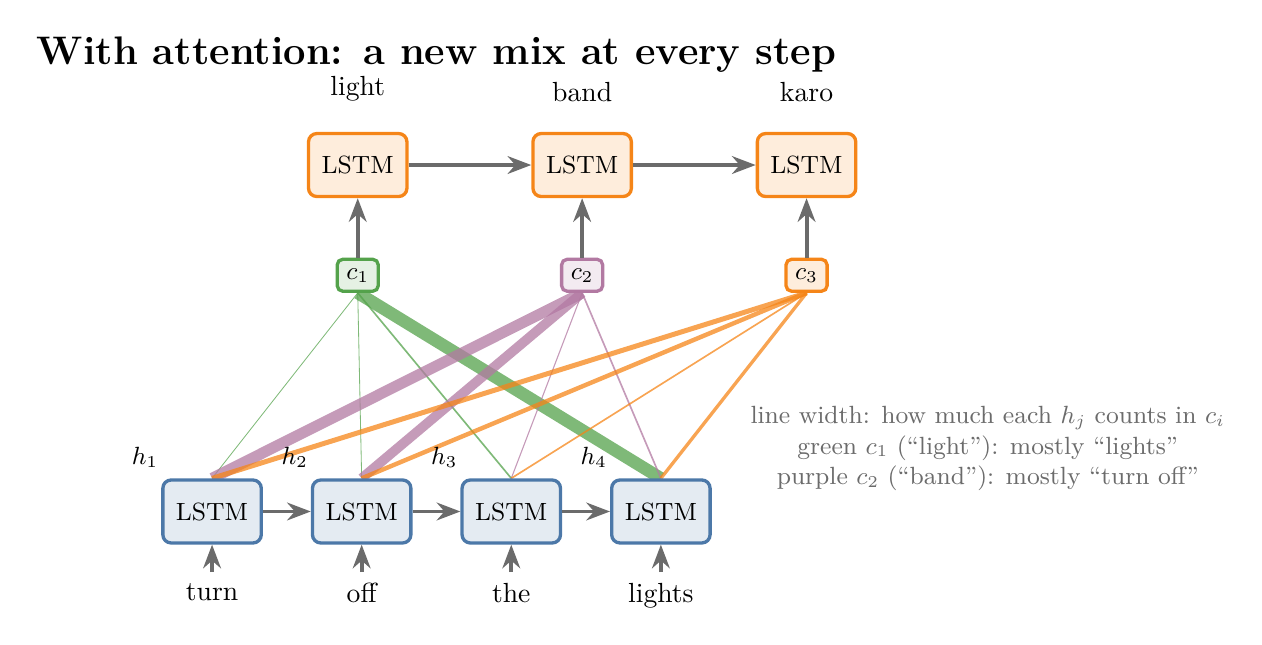
\begin{tikzpicture}[cell/.style={draw=#1, fill=#1!15, minimum width=1.25cm, minimum height=0.8cm, rounded corners=3pt, font=\sffamily\small},
  word/.style={font=\sffamily}]
  \node[title] at (4.75, 5.8) {With attention: a new mix at every step};
  \foreach \w [count=\j] in {turn, off, the, lights} {
    \node[cell=cblue] (e\j) at (1.9*\j, 0) {LSTM};
    \node[word, below=0.35cm of e\j] (x\j) {\w};
    \draw[arrow] (x\j) -- (e\j);
    \node[font=\sffamily\small, above left=0.0cm and -0.1cm of e\j] {$h_\j$};
  }
  \foreach \i/\j in {1/2, 2/3, 3/4} \draw[arrow] (e\i) -- (e\j);
  \foreach \w/\a/\b/\c/\d/\col [count=\i] in {light/0.3/0.3/0.6/4.5/cgreen, band/4.0/3.5/0.4/0.6/cpurple, karo/1.8/1.6/0.6/1.2/corange} {
    \node[draw=\col, fill=\col!15, rounded corners=2pt, font=\sffamily\small] (c\i) at (1.9 + 2.85*\i - 1.0, 3.0) {$c_\i$};
    \node[cell=corange] (d\i) at (1.9 + 2.85*\i - 1.0, 4.4) {LSTM};
    \node[word, above=0.25cm of d\i] {\w};
    \draw[arrow] (c\i) -- (d\i);
    \begin{scope}[on background layer]
    \draw[draw=\col, line width=\a pt, opacity=0.75] (e1.north) -- (c\i.south);
    \draw[draw=\col, line width=\b pt, opacity=0.75] (e2.north) -- (c\i.south);
    \draw[draw=\col, line width=\c pt, opacity=0.75] (e3.north) -- (c\i.south);
    \draw[draw=\col, line width=\d pt, opacity=0.75] (e4.north) -- (c\i.south);
    \end{scope}
  }
  \draw[arrow] (d1) -- (d2); \draw[arrow] (d2) -- (d3);
  \node[note, anchor=west] at (8.6, 0.8) {line width: how much each $h_j$ counts in $c_i$\\green $c_1$ (``light''): mostly ``lights''\\purple $c_2$ (``band''): mostly ``turn off''};
\end{tikzpicture}
\end{document}
